\documentclass[11pt]{article}

\usepackage[utf8]{inputenc}
\usepackage[T1]{fontenc}
\usepackage{amsmath,amssymb}
\usepackage{graphicx}
\usepackage{booktabs}
\usepackage[hidelinks]{hyperref}
\usepackage{float}
\usepackage[colorinlistoftodos]{todonotes}
\usepackage{tikz}
\usetikzlibrary{arrows.meta, positioning}
\usepackage[margin=0.75in]{geometry}
\usepackage[compact]{titlesec}
\usepackage{enumitem}
\setlist{nosep}

\title{Lexical BM25, Dense Vector Retrieval (HNSW), and Two-Stage Re-ranking\\[0.5em]
    \large CS6913: Web Search Engines --- Assignment \#3}
\author{
    Anna Gardner\\
    \texttt{ag7618@nyu.edu}
    \and
    Alexander Sanchez\\
    \texttt{fas6501@nyu.edu}
}
\date{}

\begin{document}

\maketitle

\begin{abstract}
We evaluate and compare three information retrieval architectures on a 1,000,000-passage subset of the MS-MARCO corpus: (1) a compressed block-encoded BM25 inverted index in Rust supporting disjunctive (\texttt{OR}) and conjunctive (\texttt{AND}) Document-at-a-Time (DAAT) query processing, (2) an in-memory Hierarchical Navigable Small World (\texttt{faiss.IndexHNSWFlat}) dense vector index over 384-dimensional embeddings using inner-product similarity, and (3) a two-stage hybrid cascade that retrieves the top-$1{,}000$ BM25 candidates and re-ranks them via exact vector dot products. Across 36 HNSW hyperparameter configurations spanning $(M, \mathit{efConstruction}, \mathit{efSearch})$ from $(4, 50, 50)$ to $(8, 200, 200)$, we analyze index build time, memory scaling, multi-threaded hardware efficiency, and retrieval quality on TREC DL 2019 (\texttt{eval.one}), TREC DL 2020 (\texttt{eval.two}), and MS-MARCO \texttt{dev}. We show that while sparse HNSW graphs ($M=4$) suffer from local minima, well-connected HNSW graphs ($M \in \{6,7,8\}$) achieve sub-$0.1\,\text{ms/query}$ latency and outperform standalone BM25 by $+54.84\%$ in NDCG@10. Finally, two-stage hybrid re-ranking achieves the highest overall precision on \texttt{eval.one} ($\text{MRR@10}=0.9651$, $\text{NDCG@10}=0.7053$) and \texttt{dev} ($\text{MRR@10}=0.5843$, $\text{Recall@100}=0.8933$), whereas standalone HNSW slightly outperforms hybrid re-ranking on \texttt{eval.two} ($\text{NDCG@10}=0.6655$ vs.\ $0.6578$) by overcoming first-stage lexical vocabulary mismatch.
\end{abstract}

% =============================================================================
\section{Overview and Experimental Setup}
% =============================================================================

Lexical retrieval models such as BM25 excel at exact keyword and rare-entity matching using compact inverted indexes, but fail when queries and relevant passages use different vocabulary (synonyms or paraphrases). Dense vector retrieval addresses this lexical gap by encoding queries and passages into a shared $384$-dimensional embedding space and scoring relevance via inner-product similarity. In this report, we compare standalone lexical search (System~\#1), standalone approximate nearest neighbor (ANN) vector search via HNSW (System~\#2), and a two-stage lexical-then-dense re-ranking pipeline (System~\#3), illustrated in Figure~\ref{fig:arch}.

\begin{figure}[H]
\centering
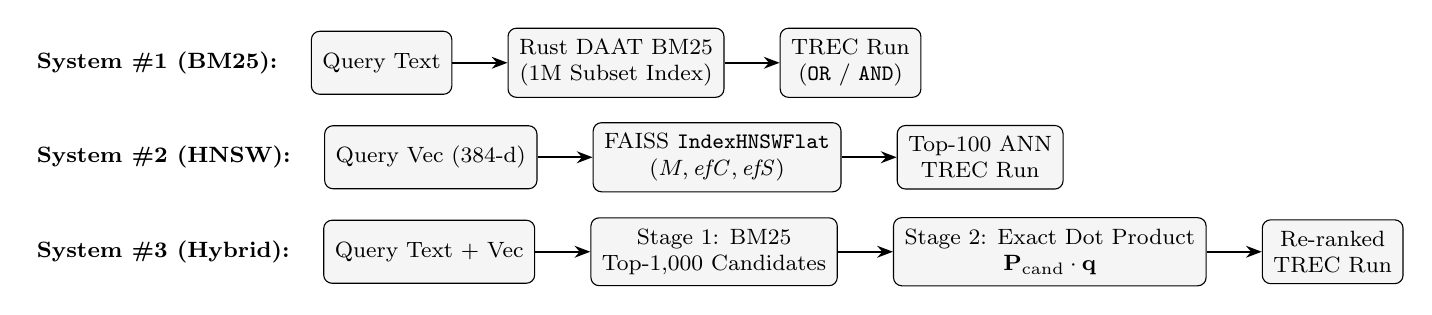
\begin{tikzpicture}[
    node distance=0.45cm and 0.7cm,
    box/.style={draw, rounded corners=3pt, align=center, font=\footnotesize, minimum height=0.8cm, inner sep=4pt, fill=gray!8},
    arr/.style={-{Stealth[length=2mm]}, thick}
]
    % System 1
    \node[font=\footnotesize\bfseries, anchor=west] (s1_lbl) at (0, 1.4) {System \#1 (BM25):};
    \node[box, right=0.3cm of s1_lbl] (s1_q) {Query Text};
    \node[box, right=of s1_q] (s1_idx) {Rust DAAT BM25\\(1M Subset Index)};
    \node[box, right=of s1_idx] (s1_out) {TREC Run\\(\texttt{OR} / \texttt{AND})};
    \draw[arr] (s1_q) -- (s1_idx);
    \draw[arr] (s1_idx) -- (s1_out);

    % System 2
    \node[font=\footnotesize\bfseries, anchor=west] (s2_lbl) at (0, 0.2) {System \#2 (HNSW):};
    \node[box, right=0.3cm of s2_lbl] (s2_q) {Query Vec ($384$-d)};
    \node[box, right=of s2_q] (s2_idx) {FAISS \texttt{IndexHNSWFlat}\\$(M, \mathit{efC}, \mathit{efS})$};
    \node[box, right=of s2_idx] (s2_out) {Top-100 ANN\\TREC Run};
    \draw[arr] (s2_q) -- (s2_idx);
    \draw[arr] (s2_idx) -- (s2_out);

    % System 3
    \node[font=\footnotesize\bfseries, anchor=west] (s3_lbl) at (0, -1.0) {System \#3 (Hybrid):};
    \node[box, right=0.3cm of s3_lbl] (s3_q) {Query Text + Vec};
    \node[box, right=of s3_q] (s3_s1) {Stage 1: BM25\\Top-$1{,}000$ Candidates};
    \node[box, right=of s3_s1] (s3_s2) {Stage 2: Exact Dot Product\\$\mathbf{P}_{\text{cand}} \cdot \mathbf{q}$};
    \node[box, right=of s3_s2] (s3_out) {Re-ranked\\TREC Run};
    \draw[arr] (s3_q) -- (s3_s1);
    \draw[arr] (s3_s1) -- (s3_s2);
    \draw[arr] (s3_s2) -- (s3_out);
\end{tikzpicture}
\caption{Architecture of the three retrieval systems evaluated on the 1M MS-MARCO passage subset.}
\label{fig:arch}
\end{figure}

\subsection{Dataset Filtering and 1M Subset Preparation}
Because HNSW keeps uncompressed embedding vectors and graph adjacency lists in RAM, indexing all $8{,}841{,}823$ MS-MARCO passages would require $\sim 13.6\,\text{GB}$ for raw vectors alone. Using \texttt{subset\_processor.py}, we loaded the $1{,}000{,}000$ target passage IDs from \texttt{msmarco\_passages\_subset.tsv} into a Python \texttt{set} ($O(1)$ membership lookup) and streamed the full $8.8\text{M}$ \texttt{collection.tsv} to extract \texttt{collection\_subset.tsv} ($345.7\,\text{MB}$, exactly $1{,}000{,}000$ passages).

Passage and query embeddings were loaded from \texttt{msmarco\_passages\_embeddings\_subset.h5} ($1{,}000{,}000 \times 384$, \texttt{float32}) and \texttt{msmarco\_queries\_dev\_eval\_embeddings.h5} ($202{,}185 \times 384$, \texttt{float32}) via \texttt{read\_h5.py}, decoding UTF-8 ID strings and enforcing C-contiguous \texttt{np.float32} memory layout for FAISS C++ interoperability.

\subsection{Evaluation Benchmarks and Judging Characteristics}
All three systems output rankings in standard 6-column TREC format (\texttt{qid Q0 docid rank score tag}) and are evaluated via \texttt{score.py} wrapping \texttt{trec\_eval -c}. Table~\ref{tab:benchmarks} summarizes the three evaluation sets.

\begin{table}[H]
\centering
\resizebox{\textwidth}{!}{%
\begin{tabular}{llrrll}
\toprule
\textbf{Benchmark} & \textbf{Qrels File} & \textbf{Queries} & \textbf{Total Judgments} & \textbf{Relevance Scale} & \textbf{Evaluated Metrics} \\
\midrule
TREC DL 2019 & \texttt{qrels.eval.one.tsv} & 43 & 9,260 ($\sim 215.3$/q) & Graded ($0, 1, 2, 3$) & MRR@10, Recall@100, NDCG@10, NDCG@100 \\
TREC DL 2020 & \texttt{qrels.eval.two.tsv} & 54 & 11,386 ($\sim 210.9$/q) & Graded ($0, 1, 2, 3$) & MRR@10, Recall@100, NDCG@10, NDCG@100 \\
MS-MARCO Dev & \texttt{qrels.dev.tsv} & 1,000 & 1,073 ($\sim 1.07$/q) & Binary ($1$ only) & MRR@10, Recall@100, MAP \\
\bottomrule
\end{tabular}%
}
\caption{Summary of query evaluation sets and relevance judgment characteristics.}
\label{tab:benchmarks}
\end{table}


Crucially, \texttt{eval.one} and \texttt{eval.two} feature deep NIST pooling ($\sim 210$ human-graded passages per query across four relevance grades $0$--$3$), making NDCG@10 and NDCG@100 highly informative measures of multi-level ranking quality. By contrast, \texttt{qrels.dev.tsv} provides sparse binary judgments ($\sim 1.07$ judged relevant passages per query) and has only 3 columns (\texttt{qid docid rel}); \texttt{score.py} automatically injects the missing second TREC \texttt{0} column into a temporary file and evaluates MAP instead of NDCG.

% =============================================================================
\section{System Implementations}
% =============================================================================

\subsection{System \#1: Rebuilt BM25 Index and Batch Candidate Exporter}
We rebuilt our Assignment~\#2 Rust inverted index on \texttt{collection\_subset.tsv} ($N = 1{,}000{,}000$ documents, $54{,}344{,}449$ total tokens, average length $\text{avgdl} = 54.34$ tokens). The resulting on-disk index occupies $109.671\,\text{MB}$ total ($68.983\,\text{MB}$ \texttt{postings.bin}, $14.871\,\text{MB}$ \texttt{lexicon.bin}, $17.818\,\text{MB}$ \texttt{doc\_table.tsv}, $8.000\,\text{MB}$ \texttt{passage\_offsets.bin}, and $83\,\text{B}$ \texttt{collection\_stats.json}).

To export candidate runs for Assignment~\#3, we added \texttt{crates/query/src/batch.rs} (\texttt{query --batch}), which filters \texttt{queries.dev.tsv} and \texttt{queries.eval.tsv} down to the judged query IDs in each \texttt{qrels} file, disables passage snippet disk reads (\texttt{engine.disable\_snippets()}), and exports top-$K=1{,}000$ rankings under both disjunctive (\texttt{OR}) and conjunctive (\texttt{AND}) query modes.

Using a MacBook Air computer with the Apple M3 chip (8 CPU cores and 16 GB of RAM), for each evaluation set and query mode, we used a single sequential release-build batch with snippets disabled and $K$ set to $1{,}000$. In the latest run, the $1{,}000$ \texttt{dev} queries required $12.194\,\text{s}$ for \texttt{OR} export and generated $998{,}299$ rows of output, whereas \texttt{AND} required $0.037\,\text{s}$ and gave $1{,}708$ rows of output. For the $43$ \texttt{eval.one} queries, \texttt{OR} took $0.536\,\text{s}$ to get $43{,}000$ rows of output, and \texttt{AND} required $0.007\,\text{s}$ for $128$ rows of output; for the $54$ \texttt{eval.two} queries, \texttt{OR} required $0.585\,\text{s}$ to get $54{,}000$ rows of output and \texttt{AND} required $0.009\,\text{s}$ to produce $59$ rows of output. These latest-run timings are used consistently in the tables. Note that the batch-export times include time spent on qrels loading, filtering by query, search, and writing the run; the timings do not include index initialization time. The timings measured are elapsed times for each complete batch rather than individual-query response latencies.

\subsection{System \#2: Dense Vector Retrieval with FAISS HNSW}
In \texttt{hnsw\_search.py}, we first filter the $202{,}185$ query embeddings down to the exact unique query IDs present in each \texttt{qrels} file ($43$, $54$, and $1{,}000$ queries) via $O(1)$ dictionary row mapping. We construct an in-memory \texttt{faiss.IndexHNSWFlat(384, m, faiss.METRIC\_INNER\_PRODUCT)} index, explicitly setting \texttt{index.hnsw.efConstruction} prior to calling \texttt{index.add(passage\_embeddings)}. At query time, we set \texttt{index.hnsw.efSearch}, retrieve the top $k=100$ nearest neighbors via \texttt{index.search()}, map FAISS internal row indices ($0 \dots 999{,}999$) back to external MS-MARCO passage IDs, and write 6-column TREC run files.

\subsection{System \#3: Two-Stage BM25 + Exact Vector Re-ranking}
In \texttt{rerank.py}, Stage~1 reads the candidate passage IDs per query from a 6-column BM25 run file (\texttt{bm25\_*.run} for \texttt{OR} and \texttt{bm25\_and\_*.run} for \texttt{AND}, up to $K=1{,}000$ candidates per query). Stage~2 maps the query ID and its candidate passage IDs to their row indices in the pre-loaded \texttt{.h5} embedding matrices, computes exact inner-product scores via vectorized matrix-vector multiplication (\texttt{scores = passage\_vectors[rows] @ qvec}), sorts the candidates in descending order of dot product, and writes the re-ranked TREC run file.

The candidate count $K$ determines how many BM25 passages per query receive exact vector scores; the final Recall@100 is still based on looking only at the first $100$ re-ranked passages. Evaluation uses \texttt{trec\_eval -c} to ensure that a judged query with no \texttt{AND} candidates remains in the denominator. For the three-column \texttt{dev} qrels, \texttt{score.py} inserts the required second TREC column before scoring, and reports MAP instead of NDCG.

% =============================================================================
\section{HNSW Hyperparameter Exploration and Efficiency Analysis}
% =============================================================================

HNSW graph construction and search are governed by three hyperparameters:
\begin{itemize}
    \item \textbf{$M$ (Graph Degree):} Number of bidirectional neighbor links per node ($2M$ at layer $0$). Controls graph connectivity and RAM overhead.
    \item \textbf{$\mathit{efConstruction}$ (Construction Beam Width):} Candidate priority-queue size during \texttt{index.add()}. Higher values yield better-connected graphs at the cost of longer build times, without altering memory footprint.
    \item \textbf{$\mathit{efSearch}$ (Search Beam Width):} Candidate priority-queue size during \texttt{index.search()}. Trades query latency against recall without rebuilding the index.
\end{itemize}
We swept 9 graph configurations across $M \in \{4, 5, 6, 7, 8\}$ and $\mathit{efConstruction} \in \{50, 100, 150, 200\}$, evaluating each across $\mathit{efSearch} \in \{50, 100, 150, 200\}$ ($36$ total configurations per query set).

\subsection{Index Construction Time and Memory Footprint}
We measured exact index memory by summing the raw \texttt{float32} vector buffer ($1{,}000{,}000 \times 384 \times 4\text{ B} = 1{,}464.84\,\text{MB}$) and FAISS's internal HNSW graph arrays (\texttt{neighbors} at $4\text{ B}$, \texttt{offsets} at $8\text{ B}$, and \texttt{levels} at $4\text{ B}$). Table~\ref{tab:hnsw_mem} reports build times and memory footprints.

\begin{table}[H]
\centering
\resizebox{\textwidth}{!}{%
\begin{tabular}{lrrrrr}
\toprule
\textbf{Graph Config $(M, \mathit{efConstruction})$} & \textbf{Build Time (s)} & \textbf{Rel.\ Build Time} & \textbf{Total RAM (MB)} & \textbf{Graph RAM (MB)} & \textbf{Graph Bytes / Vec} \\
\midrule
$(M=4, \mathit{efC}=50)$  & 42.97 s  & $1.00\times$ & 1,511.89 MB & 47.04 MB & 49.3 B \\
$(M=4, \mathit{efC}=100)$ & 71.54 s  & $1.66\times$ & 1,511.89 MB & 47.04 MB & 49.3 B \\
$(M=4, \mathit{efC}=150)$ & 94.08 s  & $2.19\times$ & 1,511.89 MB & 47.04 MB & 49.3 B \\
$(M=5, \mathit{efC}=100)$ & 89.27 s  & $2.08\times$ & 1,519.19 MB & 54.35 MB & 57.0 B \\
$(M=5, \mathit{efC}=150)$ & 116.66 s & $2.71\times$ & 1,519.19 MB & 54.35 MB & 57.0 B \\
$(M=6, \mathit{efC}=100)$ & 102.67 s & $2.39\times$ & 1,526.63 MB & 61.78 MB & 64.8 B \\
$(M=6, \mathit{efC}=150)$ & 141.19 s & $3.29\times$ & 1,526.63 MB & 61.78 MB & 64.8 B \\
$(M=7, \mathit{efC}=150)$ & 168.04 s & $3.91\times$ & 1,534.13 MB & 69.29 MB & 72.7 B \\
$(M=8, \mathit{efC}=200)$ & 237.49 s & $5.53\times$ & 1,541.68 MB & 76.83 MB & 80.6 B \\
\bottomrule
\end{tabular}%
}
\caption{HNSW index build time and exact memory breakdown across $(M, \mathit{efConstruction})$ configurations on 1M vectors.}
\label{tab:hnsw_mem}
\end{table}

Two structural laws emerge from Table~\ref{tab:hnsw_mem}:
\begin{enumerate}
    \item \textbf{Graph RAM scales strictly linearly with $M$ and is invariant to $\mathit{efConstruction}$:} Every $+1$ increase in $M$ ($4 \to 5 \to 6 \to 7 \to 8$) adds almost exactly $+7.45\,\text{MB}$ ($\sim 7.8\text{ bytes/vector}$) to the HNSW graph. Even at $M=8$, the graph structure ($76.83\,\text{MB}$) accounts for just $4.98\%$ of total index memory ($1{,}541.68\,\text{MB}$).
    \item \textbf{Build time scales super-linearly with $(M, \mathit{efConstruction})$:} Increasing $(4, 50) \to (8, 200)$ increases build time by $5.53\times$ ($42.97\,\text{s} \to 237.49\,\text{s}$), as each inserted node performs a wider greedy beam search and prunes candidate edges across larger neighbor lists.
\end{enumerate}

\subsection{Retrieval Quality vs.\ Query Latency Across the 36-Configuration Grid}
Rather than listing all 36 HNSW configurations in full, Table~\ref{tab:hnsw_sweep} presents 10 representative HNSW operating points spanning $M \in \{4, 5, 6, 7, 8\}$ alongside standalone BM25 and two-stage re-ranking across all three benchmarks. Across the complete 36-configuration grid, per-query search latency ranged from $0.028\,\text{ms/q}$ at $(4, 150, 50)$ on \texttt{eval.one} up to $0.184\,\text{ms/q}$ at $(8, 200, 200)$ on \texttt{dev} (with a brief one-off OS scheduling spike of $0.241$--$0.281\,\text{ms/q}$ on the 43-query \texttt{eval.one} micro-batch at $(5, 100, \mathit{efS} \in \{100, 150, 200\})$). Within each graph $(M, \mathit{efConstruction})$, increasing $\mathit{efSearch}$ from $50 \to 100 \to 150 \to 200$ monotonically increased query latency by roughly $2\times$--$3.3\times$ while yielding progressively smaller recall and ranking gains once graph connectivity saturated.

\begin{table}[H]
\centering
\resizebox{\textwidth}{!}{%
\setlength{\tabcolsep}{3.5pt}
\begin{tabular}{l|rrrrr|rrrrr|rrrr}
\toprule
& \multicolumn{5}{c|}{\textbf{TREC DL 2019 (\texttt{eval.one}, 43q)}} & \multicolumn{5}{c|}{\textbf{TREC DL 2020 (\texttt{eval.two}, 54q)}} & \multicolumn{4}{c}{\textbf{MS-MARCO \texttt{dev} (1,000q)}} \\
\textbf{System / $(M,\mathit{efC},\mathit{efS})$} & \textbf{ms/q} & \textbf{MRR@10} & \textbf{R@100} & \textbf{NDCG@10} & \textbf{NDCG@100} & \textbf{ms/q} & \textbf{MRR@10} & \textbf{R@100} & \textbf{NDCG@10} & \textbf{NDCG@100} & \textbf{ms/q} & \textbf{MRR@10} & \textbf{R@100} & \textbf{MAP} \\
\midrule
BM25 (\texttt{OR}, top 1000) & 12.4651 & 0.7942 & 0.5174 & 0.4517 & 0.5335 & 10.8333 & 0.8148 & 0.5251 & 0.4985 & 0.5144 & 12.1940 & 0.3990 & 0.8050 & 0.4016 \\
BM25 (\texttt{AND})          & 0.1628 & 0.4070 & 0.0240 & 0.1293 & 0.0619 & 0.1667 & 0.3426 & 0.0250 & 0.1124 & 0.0619 & 0.0370 & 0.0951 & 0.1063 & 0.0924 \\
\midrule
HNSW $(4, 50, 50)$   & 0.040 & 0.6705 & 0.3418 & 0.4535 & 0.4083 & 0.039 & 0.6730 & 0.3621 & 0.4567 & 0.4056 & 0.029 & 0.2634 & 0.4327 & 0.2606 \\
HNSW $(4, 50, 200)$  & 0.081 & 0.8845 & 0.4570 & 0.6111 & 0.5601 & 0.079 & 0.8767 & 0.4602 & 0.5916 & 0.5227 & 0.107 & 0.3616 & 0.5847 & 0.3586 \\
HNSW $(4, 100, 100)$ & 0.051 & 0.8845 & 0.5139 & 0.6247 & 0.6079 & 0.051 & 0.8397 & 0.5099 & 0.6064 & 0.5562 & 0.053 & 0.3763 & 0.6188 & 0.3739 \\
HNSW $(4, 150, 100)$ & 0.054 & 0.7915 & 0.4743 & 0.5665 & 0.5564 & 0.053 & 0.8582 & 0.5244 & 0.6033 & 0.5657 & 0.052 & 0.3994 & 0.6540 & 0.3955 \\
HNSW $(5, 100, 50)$  & 0.042 & 0.7868 & 0.4436 & 0.5740 & 0.5439 & 0.063 & 0.8611 & 0.5484 & 0.6262 & 0.5846 & 0.045 & 0.3942 & 0.6478 & 0.3933 \\
HNSW $(5, 150, 100)$ & 0.064 & 0.9078 & 0.5319 & 0.6605 & 0.6265 & 0.062 & 0.9230 & 0.5995 & 0.6548 & 0.6228 & 0.063 & 0.4536 & 0.7365 & 0.4523 \\
HNSW $(6, 150, 50)$  & 0.037 & 0.8837 & 0.5242 & 0.6274 & 0.6106 & 0.052 & \textbf{0.9323} & 0.6128 & \textbf{0.6655} & 0.6356 & 0.042 & 0.4509 & 0.7330 & 0.4487 \\
HNSW $(7, 150, 50)$  & 0.041 & 0.9070 & 0.5078 & 0.6588 & 0.6137 & 0.049 & 0.9230 & \textbf{0.6141} & 0.6625 & \textbf{0.6391} & 0.047 & 0.4887 & 0.7799 & 0.4866 \\
HNSW $(8, 200, 50)$  & 0.046 & 0.9535 & 0.5499 & 0.6994 & 0.6550 & 0.044 & 0.9045 & 0.6019 & 0.6500 & 0.6259 & 0.055 & 0.5072 & 0.8111 & 0.5058 \\
HNSW $(8, 200, 100)$ & 0.072 & 0.9535 & 0.5564 & 0.6987 & 0.6557 & 0.092 & 0.9230 & 0.6112 & 0.6627 & 0.6377 & 0.095 & 0.5427 & 0.8599 & 0.5414 \\
HNSW $(8, 200, 200)$ & 0.130 & 0.9535 & 0.5557 & 0.6987 & 0.6544 & 0.131 & 0.9230 & 0.6056 & 0.6627 & 0.6343 & 0.184 & 0.5603 & 0.8909 & 0.5592 \\
\midrule
BM25 (\texttt{OR}) + Rerank  & 14.2054 & \textbf{0.9651} & \textbf{0.5689} & \textbf{0.7053} & \textbf{0.6619} & 12.4396 & 0.9259 & 0.6111 & 0.6578 & 0.6339 & 13.8342 & \textbf{0.5843} & \textbf{0.8933} & \textbf{0.5815} \\
BM25 (\texttt{AND}) + Rerank & 0.2151 & 0.3845 & 0.0240 & 0.1323 & 0.0618 & 0.2117 & 0.3519 & 0.0250 & 0.1153 & 0.0638 & 0.0855 & 0.1022 & 0.1063 & 0.0988 \\
\bottomrule
\end{tabular}%
}
\caption{Retrieval quality and amortized batch time across BM25, representative HNSW configurations (from the 36-configuration sweep), and two-stage re-ranking. BM25 and hybrid timings use the latest runs, include run I/O, and exclude initialization; HNSW sweep timings cover search only on a separate machine.}
\label{tab:hnsw_sweep}
\end{table}

In the BM25 \texttt{OR} rows, ``top 1,000'' means the candidate-pool size that was exported. Each of the R@100 columns measures Recall@100 while using only the first $100$ ranked passages. The raw BM25 values are $0.8050$ on \texttt{dev}, $0.5174$ on \texttt{eval.one}, and $0.5251$ on \texttt{eval.two}. The $80.5\%$ value on \texttt{dev} therefore refers specifically to Recall@100, not recall over the full $1{,}000$-candidate pool.

\textbf{Key Insights from the Hyperparameter Sweep:}
\begin{enumerate}
    \item \textbf{Graph Connectivity ($M$) vs.\ Search Beam Width ($\mathit{efSearch}$):} At $(4, 50, 50)$, HNSW achieves only $0.4327$ Recall@100 on \texttt{dev} and $0.3418$ on \texttt{eval.one} because $M=4$ leaves the proximity graph poorly connected, causing greedy search to get trapped in local minima. Even when pushing $\mathit{efSearch}$ to $200$ on the $(4, 50)$ graph ($\text{Recall@100} = 0.5847$ at $0.107\,\text{ms/q}$ on \texttt{dev}), it is outperformed by $(5, 100, 50)$ ($\text{Recall@100} = 0.6478$ at $0.045\,\text{ms/q}$), which is both $2.38\times$ faster and $+6.3\%$ more accurate.
    \item \textbf{Saturation of $\mathit{efConstruction}$ at Low $M$:} At $M=4$, raising $\mathit{efConstruction}$ from $50 \to 100$ substantially improves \texttt{dev} Recall@100 ($0.5097 \to 0.6188$ at $\mathit{efS}=100$), but further increasing $\mathit{efConstruction}$ to $150$ yields diminishing returns ($0.6188 \to 0.6540$) because 4 neighbor slots per node saturate quickly. Higher $M \in \{6, 7, 8\}$ pairs synergistically with $\mathit{efConstruction} \in \{150, 200\}$.
    \item \textbf{Early Saturation on Graded Eval Sets vs.\ Continuous Gains on Sparse Dev:} On $(8, 200)$, \texttt{eval.one} and \texttt{eval.two} reach peak NDCG@10 ($0.6994$ and $0.6627$) by $\mathit{efSearch} \in [50, 100]$; increasing $\mathit{efSearch}$ to $200$ doubles latency ($0.095 \to 0.184\,\text{ms/q}$) without improving NDCG@10. On \texttt{dev}, where each query targets a single sparse passage, increasing $\mathit{efSearch}$ from $50 \to 200$ steadily lifts Recall@100 ($0.8111 \to 0.8909$) and MRR@10 ($0.5072 \to 0.5603$).
\end{enumerate}

\subsection{Hardware Scaling and Multi-Threading Dynamics}
We additionally benchmarked HNSW build and search performance across two hardware platforms: Machine~\#1 (Intel Core i7-7500U, 2 cores / 4 threads, 15W TDP, Fedora Linux \texttt{libgomp}) and Machine~\#2 (Intel Core i9-8950HK, 6 cores / 12 threads, 45W TDP, macOS \texttt{libomp}):
\begin{itemize}
    \item \textbf{Memory-Wall Bound Construction:} Although Machine~\#2 has $3\times$ the physical cores of Machine~\#1, $(4, 50)$ index construction is $\sim 2.15\times$ faster ($42.97\,\text{s}$ vs.\ $92.25\,\text{s}$). HNSW construction is random-access memory-bandwidth bound ($\sim 35\,\text{GB/s}$ dual-channel DDR4) and incurs lock contention when threads concurrently update bidirectional neighbor lists.
    \item \textbf{Physical Cores vs.\ Hyper-Threading:} Sweeping \texttt{faiss.omp\_set\_num\_threads()} on Machine~\#2 for the 43-query \texttt{eval.one} batch showed near-linear scaling from 1 thread ($4.78\,\text{ms}$, $0.111\,\text{ms/q}$) to 6 physical cores ($1.37\,\text{ms}$, $0.032\,\text{ms/q}$), but negligible gain at 8 or 12 hyperthreads ($1.31\,\text{ms}$, $0.031\,\text{ms/q}$, a $4.38\%$ reduction). Co-located hyperthreads executing pointer-chasing graph traversals thrash shared $32\,\text{KB}$ L1 and $256\,\text{KB}$ L2 caches.
    \item \textbf{Micro-Batch OpenMP Synchronization Tax:} On small batches (43 queries $\approx 3.5$ queries/thread on 12 threads), cold OS page faults and OpenMP barrier wakeup inflate initial latency ($7.29\,\text{ms}$ cold vs.\ $1.31\,\text{ms}$ warm), whereas the 1,000-query \texttt{dev} set amortizes thread-pool dispatch.
\end{itemize}

% =============================================================================
\section{Cross-System Analysis: Quality and Efficiency Trade-Offs}
% =============================================================================

\subsection{Retrieval Quality Comparison}
\begin{enumerate}
    \item \textbf{BM25 (\texttt{OR} vs.\ \texttt{AND}):} Disjunctive BM25 (\texttt{OR}) achieves strong broad candidate recall ($\text{Recall@100} = 0.8050$ on \texttt{dev}, $0.5174$ on \texttt{eval.one}), confirming that most relevant passages share at least one keyword with the query. However, its top-10 ranking precision ($\text{NDCG@10} = 0.4517$ on \texttt{eval.one}, $\text{MRR@10} = 0.3990$ on \texttt{dev}) trails dense vector retrieval because exact term frequency cannot capture semantic similarity. Conjunctive BM25 (\texttt{AND}) collapses ($\text{Recall@100} = 0.0240$ on \texttt{eval.one}, $0.1063$ on \texttt{dev}) because requiring all 6--10 query tokens to appear in a 54-word passage eliminates nearly all relevant documents.
    \item \textbf{Why Two-Stage Re-ranking Wins on \texttt{eval.one} and \texttt{dev}:} Re-ranking BM25 \texttt{OR}'s top-$1{,}000$ candidates with exact vector inner products boosts \texttt{eval.one} NDCG@10 by $+56.1\%$ ($0.4517 \to 0.7053$) and \texttt{dev} MRR@10 by $+46.4\%$ ($0.3990 \to 0.5843$). Notably, Recall@100 also rises substantially after re-ranking ($0.5174 \to 0.5689$ on \texttt{eval.one}; $0.8050 \to 0.8933$ on \texttt{dev}) because relevant passages ranked between positions $101$ and $1{,}000$ by BM25 are promoted into the top 100 by their dense dot-product scores. Conversely, \texttt{reranked\_and} exhibits identical Recall@100 to \texttt{bm25\_and} ($0.0240$ / $0.1063$), demonstrating that a second-stage re-ranker is strictly bounded by first-stage recall.
    \item \textbf{When Standalone HNSW Beats Two-Stage Re-ranking (\texttt{eval.two}):} On \texttt{eval.two}, standalone HNSW at $(6, 150, 50)$, $(7, 150, 50)$, and $(8, 200, 100)$ outperforms \texttt{BM25 (OR) + Rerank} in NDCG@10 ($0.6655$ vs.\ $0.6578$), NDCG@100 ($0.6391$ vs.\ $0.6339$), and Recall@100 ($0.6141$ vs.\ $0.6111$). When relevant passages use synonyms or paraphrases with zero lexical overlap with the query, Stage-1 BM25 fails to include them in the top-$1{,}000$ pool, whereas HNSW searches the entire 1M vector space directly.
\end{enumerate}

\subsection{Trade-Offs Between Re-ranking and BM25 Candidate Count}
Table~\ref{tab:rerank_k} shows the complete candidate-count experiment. Each numbered row re-ranks the top $K$ BM25 \texttt{OR} candidates; the HNSW control returns $100$ passages directly. The HNSW control from the candidate-count table was run on a different machine and used a different index build from the HNSW hyperparameter sweep. All recall values in this table, regardless of the candidate count, are Recall@100.

\begin{table}[H]
\centering
\small
\begin{tabular}{llrrrrr}
\toprule
\textbf{Benchmark} & \textbf{$K$ / control} & \textbf{MRR@10} & \textbf{Recall@100} & \textbf{NDCG@10} & \textbf{NDCG@100} & \textbf{MAP} \\
\midrule
\texttt{eval.one} & 10 & 0.8718 & 0.1343 & 0.5000 & 0.2423 & --- \\
 & 20 & 0.9180 & 0.2123 & 0.6075 & 0.3392 & --- \\
 & 50 & 0.9388 & 0.3780 & 0.6715 & 0.4845 & --- \\
 & 100 & 0.9612 & 0.5174 & 0.6899 & 0.5999 & --- \\
 & 200 & 0.9806 & 0.5487 & 0.7135 & 0.6423 & --- \\
 & 500 & 0.9690 & 0.5689 & 0.7101 & 0.6615 & --- \\
 & 1,000 & 0.9651 & 0.5689 & 0.7053 & 0.6619 & --- \\
 & HNSW & 0.9535 & 0.5567 & 0.6987 & 0.6559 & --- \\
\midrule
\texttt{eval.two} & 10 & 0.8614 & 0.1613 & 0.5228 & 0.2907 & --- \\
 & 20 & 0.8995 & 0.2520 & 0.5739 & 0.3717 & --- \\
 & 50 & 0.9213 & 0.3934 & 0.6167 & 0.4822 & --- \\
 & 100 & 0.9204 & 0.5251 & 0.6418 & 0.5800 & --- \\
 & 200 & 0.9204 & 0.5694 & 0.6556 & 0.6081 & --- \\
 & 500 & 0.9241 & 0.6019 & 0.6591 & 0.6281 & --- \\
 & 1,000 & 0.9259 & 0.6111 & 0.6578 & 0.6339 & --- \\
 & HNSW & 0.9230 & 0.6113 & 0.6627 & 0.6377 & --- \\
\midrule
\texttt{dev} & 10 & 0.5007 & 0.6028 & --- & --- & 0.4930 \\
 & 20 & 0.5282 & 0.6783 & --- & --- & 0.5210 \\
 & 50 & 0.5523 & 0.7578 & --- & --- & 0.5474 \\
 & 100 & 0.5664 & 0.8050 & --- & --- & 0.5615 \\
 & 200 & 0.5735 & 0.8420 & --- & --- & 0.5693 \\
 & 500 & 0.5792 & 0.8758 & --- & --- & 0.5762 \\
 & 1,000 & 0.5843 & 0.8933 & --- & --- & 0.5815 \\
 & HNSW & 0.5431 & 0.8599 & --- & --- & 0.5418 \\
\bottomrule
\end{tabular}
\caption{BM25 \texttt{OR} plus vector re-ranking across candidate counts, with a fixed HNSW $(8,200,100)$ control from the candidate-count experiment.}
\label{tab:rerank_k}
\end{table}

The control for fixed HNSW $(M=8,\mathit{efConstruction}=200,\mathit{efSearch}=100)$, used for the candidate-count experiment, was run from a different HNSW index build compared to the hyperparameter sweep. Its scores thus describe a separate run, despite the same configuration parameters; for example, \texttt{eval.one} Recall@100 is $0.5567$ in the candidate-count experiment, and $0.5564$ in the hyperparameter sweep.

For the candidate-count sweep of BM25 \texttt{OR}, we used $K \in \{10,20,50,100,200,500,1{,}000\}$. Raw BM25 MRR@10, and NDCG@10 on the graded eval sets, remain unchanged because every run returns at least ten passages per query. Recall@100 and NDCG@100 grow through $K=100$ because runs with $K<100$ cannot return 100 passages. Above $K=100$, those cutoff metrics are unchanged for raw BM25. The exported ranked prefixes are not identical, however, since passages with tied BM25 scores may swap order from run to run. On \texttt{dev}, raw MAP grows from $0.3921$ at $K=10$ to $0.4016$ at $K=1{,}000$ as more relevant passages enter the ranking. Re-ranking cannot change Recall@100 when $K\leq100$ because it only reorders the same candidate set. The \texttt{AND} runs return few candidates, so their metrics change little across this sweep.

On \texttt{dev}, increasing the candidate pool from $K=10$ to $1{,}000$ increases re-ranked MRR@10 from $0.5007$ to $0.5843$, Recall@100 from $0.6028$ to $0.8933$, and MAP from $0.4930$ to $0.5815$. More relevant passages become available for promotion into the final top $100$. The graded eval sets show a different trade-off at the top ranks. On \texttt{eval.one}, the re-ranked NDCG@10 peaks at $0.7135$ at $K=200$ and drops to $0.7053$ at $K=1{,}000$, while Recall@100 increases from $0.5487$ to $0.5689$. On \texttt{eval.two}, NDCG@10 peaks at $0.6591$ at $K=500$ and drops to $0.6578$ at $K=1{,}000$; Recall@100 increases from $0.6019$ to $0.6111$.

The re-ranker sorts all candidates by the vector dot product. Thus, higher $K$ may bring more relevant passages into the top $100$ while letting new candidates displace passages near the top $10$; a bigger pool does not have to make NDCG@10 better. The graded eval sets expose this difference between coverage of relevant passages and ordering of highly relevant passages. The \texttt{dev} qrels are much sparser, providing only about $1.07$ judgments per query, and so their MRR@10 and MAP track mainly where the few judged relevant passages fall. These observations describe this sweep and not a universal best $K$: \texttt{eval.one} has only $43$ queries, and \texttt{eval.two} only $54$. Scoring and sorting all the way to $K=1{,}000$ also requires more second-stage work than scoring $K=100$, with measured \texttt{OR} reranker stages of $0.20$--$0.45\,\text{ms/q}$ at $K=100$, and $1.61$--$1.74\,\text{ms/q}$ at $K=1{,}000$, across the three benchmarks.

\subsubsection{Separating Candidate Coverage from the Quality of Ranking}
The first stage can fail in two ways: it can provide no passages or it can provide passages without a judged relevant one. Both cases prevent the re-ranker from promoting a judged relevant passage. In saved \texttt{dev} runs, BM25 \texttt{OR} returns candidates for every query, but $187$ out of $1{,}000$ queries contain no judged relevant candidate passages for $K=100$. For $K=1{,}000$, this goes down to $75$. Increasing the pool from $K=100$ to $K=1{,}000$ therefore provides an additional $112$ queries with at least one judged relevant candidate. This measure of query coverage records whether any judged relevant passage is provided by the first stage. Recall@100 measures the proportion of judged relevant passages retrieved within the final first $100$ results, averaged across evaluated queries. The difference in measures matters when there are multiple relevant passages for a query.

The results of \texttt{AND} show a more constrained limit of the first stage. For example, at $K=1{,}000$, $730$ \texttt{dev} queries get no candidates, and $890$ have no judged relevant candidate. For \texttt{eval.one} and \texttt{eval.two}, the counts of empty results are $22$ of $43$ and $33$ of $54$, respectively. A faster second-stage scorer cannot fix that. This also explains why the short \texttt{AND} batch times should be considered in the context of effectiveness: the pipeline has much less to process, but it often does not have a judged relevant passage to promote. These numbers were derived from the saved BM25 runs and corresponding qrels.

This loss of query coverage follows from how \texttt{AND} uses every query term as a condition before a semantic scorer ever sees the passage. A relevant answer can include a synonym, omit wording the context implies, or have a different expression of the question. As an example, a passage that talks about the price of concrete floors can answer the question about their costs without having the word ``cost'' in it. If that word survives query preprocessing, \texttt{AND} excludes the passage no matter how semantically relevant it is. \texttt{OR} can include it through the common terms, at which point the vector scorer can check the fuller query--passage relation. This example illustrates the filtering mechanism rather than establishing the cause of every missed passage.

The two stages have different objectives: candidate retrieval must produce plausible answers, while re-ranking sorts the provided passages by their vector scores. \texttt{OR} permits more weak matches, but affords the second stage a larger pool of candidate passages. \texttt{AND} eliminates potential answers before scoring passages with vectors, and so the re-ranker does not have the opportunity to retrieve them afterward. While increasing $K$ does not soften the \texttt{AND} requirement, it does allow more passages that pass \texttt{AND}. This is why, in this experiment, larger candidate limits left the \texttt{AND} results mostly unaffected, while \texttt{OR} benefited from additional candidates. \texttt{AND} can be useful when each term indicates a necessary constraint, but matching each word does not imply relevance. In this case, the many empty \texttt{AND} results and low Recall@100 indicate that the filtering excludes too many relevant passages for these natural-language queries. Its benefits in runtime come partly from less retrieval and ranking work, rather than producing comparably relevant answers more quickly.

\subsubsection{What the Average Scores Hide}
The relatively slight changes in mean NDCG@10 do not affect every query in the same way. We used \texttt{trec\_eval -c -q -m ndcg\_cut.10} on the already re-ranked runs to inspect each query in isolation. Table~\ref{tab:query_changes} counts improvements, ties, and declines at the evaluator's four-decimal output precision. On \texttt{eval.two}, going from $K=500$ to $K=1{,}000$ changed NDCG@10 for only five queries. Three improved and two declined, but since the losses were greater than the gains, the mean score decreased. Therefore, the count of improved queries does not determine which candidate count is better.

\begin{table}[H]
\centering
\begin{tabular}{lrrrr}
\toprule
\textbf{Benchmark and change in $K$} & \textbf{Improved} & \textbf{Unchanged} & \textbf{Worsened} & \textbf{Total} \\
\midrule
\texttt{eval.one}: $200\to1{,}000$ & 6 & 28 & 9 & 43 \\
\texttt{eval.two}: $500\to1{,}000$ & 3 & 49 & 2 & 54 \\
\bottomrule
\end{tabular}
\caption{Per-query changes in re-ranked NDCG@10 when the BM25 candidate pool grows. Counts use the saved runs and four-decimal \texttt{trec\_eval} output.}
\label{tab:query_changes}
\end{table}

One concrete example is \texttt{eval.one} query $104861$, ``cost of interior concrete flooring.'' For $K=200$, the ten top-ranked passages were all at relevance grade $2$, and scored NDCG@10 of $1.0000$. For $K=1{,}000$, passage $6009067$, originally at BM25 rank $632$, moved to rank $1$ from vector scoring, yet it has relevance grade $0$. Passage $2476318$, originally at BM25 rank $352$, moves to rank $2$ from vector scoring and is unjudged. While the expanded candidate pool adds additional grade-$2$ passages into the top $10$, the first two positions receive no relevance gain in evaluation, which reduces NDCG@10 to $0.6410$. The unjudged passage should not be described as proven irrelevant, as it receives no gain simply because the qrels provided no positive judgment for it.

That single query contributes approximately $0.00835$ to the average NDCG@10 decrease across $43$ queries, which is about the same magnitude as the change in the whole average, from $0.7135$ to $0.7053$. This illustrates why we should avoid generalizing the peak observed at $K=200$ as tuning guidance. While the example depicts a real displacement of highly relevant ranked passages, the average result is still sensitive to a small number of queries. These counts are descriptive evidence, not a statistical significance test, and selecting $K$ based on these evaluations would require a separate validation set before making generalizations about performance.

\subsubsection{Metric Selection}
Different behaviors are rewarded by MRR@10, NDCG@10, and Recall@100. MRR@10 takes into account the first relevant result within ten positions, Recall@100 considers coverage across the first $100$ positions, while NDCG@10 also differentiates relevance ratings and reduces the impact of lower ranks. Thus, in this context, a candidate expansion could support a user who wants several relevant passages, even if it diminishes the quality of the initially displayed results. A high MRR@10 does not indicate that the rest of the top ten is perfectly ranked, and unchanged MRR@10 does not imply that the extra candidates produced no gain on other metrics.

The small changes from $K=500$ to $1{,}000$ demonstrate the importance of this distinction. On \texttt{dev}, MRR@10 goes up by $0.0051$, while Recall@100 increases by $0.0175$. On \texttt{eval.one}, Recall@100 remains the same at $0.5689$, while NDCG@100 rises slightly from $0.6615$ to $0.6619$ and NDCG@10 falls from $0.7101$ to $0.7053$. Thus, the additional candidates can change graded relevance and ranking without changing the number of relevant passages in the first $100$. A decision about $K$ should explain which metric matters most, rather than treating increased candidate coverage as an overall improvement.

\subsection{Time and Memory Efficiency Comparison}

\begin{table}[H]
\centering
\footnotesize
\begin{tabular}{p{0.17\textwidth}p{0.23\textwidth}p{0.25\textwidth}p{0.25\textwidth}}
\toprule
\textbf{Dimension} & \textbf{System \#1: BM25 (\texttt{OR})} & \textbf{System \#2: HNSW $(8, 200, 100)$} & \textbf{System \#3: BM25 + Vector Rerank} \\
\midrule
\textbf{Storage / RAM} & $109.67\,\text{MB}$ disk (\texttt{mmap}) & $1{,}541.7\,\text{MB}$ RAM ($1{,}464.8\text{ MB}$ vecs + $76.8\text{ MB}$ graph) & $109.67\,\text{MB}$ disk + $1{,}464.8\,\text{MB}$ vecs in RAM \\
\addlinespace[3pt]
\textbf{Build Time (1M)} & $\sim 1$--$2\,\text{min}$ (parse + merge) & $43.0\,\text{s}$ $(4,50)$ to $237.5\,\text{s}$ $(8,200)$ & $\sim 1$--$2\,\text{min}$ (BM25 only; no HNSW graph build) \\
\addlinespace[3pt]
\textbf{Query Latency} & $10.83$--$12.47\,\text{ms/q}$ (OR batch export, $K=1{,}000$) & \textbf{$0.028$--$0.281\,\text{ms/q}$} across full sweep ($0.072$--$0.095\,\text{ms/q}$ at $(8,200,100)$) & $12.44$--$14.21\,\text{ms/q}$ total; $1.61$--$1.74\,\text{ms/q}$ re-ranking and run I/O ($K=1{,}000$) \\
\addlinespace[3pt]
\textbf{Quality Profile} & Moderate recall, low top-10 precision & High recall \& precision; handles zero lexical overlap & Highest MRR@10/NDCG@10 when lexical overlap exists \\
\bottomrule
\end{tabular}
\caption{System-level trade-offs across memory, build time, query latency, and retrieval effectiveness.}
\label{tab:tradeoffs}
\end{table}

\subsubsection{Time--Quality Trade-Offs}
Table~\ref{tab:timed_rerank} provides the latest \texttt{OR} measurements on the M3 machine. The times represent batch milliseconds divided by all judged queries, including zero-result queries. BM25 includes qrels loading, query filtering, search, and writing the run; the reranker includes reading from the candidate file, vector scoring, sorting, and writing the run. Index and embedding initialization are excluded from the total measured time. Each setting was measured only once, which means that small differences in total time should not be interpreted as stable speedups.

\begin{table}[H]
\centering
\small
\begin{tabular}{lrrrr}
\toprule
\textbf{Benchmark} & \textbf{$K$} & \textbf{BM25 ms/q} & \textbf{Reranker ms/q} & \textbf{Combined ms/q} \\
\midrule
\texttt{eval.one} & 10 & 18.2093 & 0.0257 & 18.2350 \\
\texttt{eval.one} & 20 & 11.9535 & 0.0629 & 12.0164 \\
\texttt{eval.one} & 50 & 11.9767 & 0.0892 & 12.0659 \\
\texttt{eval.one} & 100 & 13.9070 & 0.4471 & 14.3541 \\
\texttt{eval.one} & 200 & 12.3256 & 0.5511 & 12.8767 \\
\texttt{eval.one} & 500 & 12.3953 & 1.0228 & 13.4181 \\
\texttt{eval.one} & 1,000 & 12.4651 & 1.7403 & 14.2054 \\
\texttt{eval.two} & 10 & 11.2222 & 0.0310 & 11.2533 \\
\texttt{eval.two} & 20 & 10.3148 & 0.0283 & 10.3431 \\
\texttt{eval.two} & 50 & 10.2593 & 0.0806 & 10.3399 \\
\texttt{eval.two} & 100 & 11.7407 & 0.2020 & 11.9427 \\
\texttt{eval.two} & 200 & 10.3704 & 0.3807 & 10.7511 \\
\texttt{eval.two} & 500 & 10.4815 & 0.8567 & 11.3382 \\
\texttt{eval.two} & 1,000 & 10.8333 & 1.6062 & 12.4396 \\
\texttt{dev} & 10 & 12.2910 & 0.0217 & 12.3127 \\
\texttt{dev} & 20 & 11.8940 & 0.0301 & 11.9241 \\
\texttt{dev} & 50 & 11.7980 & 0.0818 & 11.8798 \\
\texttt{dev} & 100 & 12.0750 & 0.2290 & 12.3040 \\
\texttt{dev} & 200 & 11.9950 & 0.4412 & 12.4362 \\
\texttt{dev} & 500 & 11.9740 & 0.8747 & 12.8487 \\
\texttt{dev} & 1,000 & 12.1940 & 1.6402 & 13.8342 \\
\bottomrule
\end{tabular}
\caption{Latest measured amortized OR pipeline times across candidate counts. Combined time is calculated from the unrounded BM25 and reranker measurements, then rounded for display.}
\label{tab:timed_rerank}
\end{table}

At $K=1{,}000$, BM25 accounts for about $87.1$--$88.1\%$ of \texttt{OR} pipeline time. The overall time rises by about $13$--$15\%$ over BM25 alone due to adding the vector reranker, while NDCG@10 improves from $0.4517$ to $0.7053$ for \texttt{eval.one} and MRR@10 from $0.3990$ to $0.5843$ for \texttt{dev}. Thus, most of the elapsed time was spent on obtaining and exporting candidates, while the additional vector stage provides substantially better ranking quality.

The optimal number of candidates depends on which quality metric matters. On \texttt{eval.one}, $K=200$ yields NDCG@10 of $0.7135$ and $0.5511\,\text{ms/q}$ of re-ranking, while $K=1{,}000$ yields $0.7053$ and $1.7403\,\text{ms/q}$. Thus, there are trade-offs: the larger pool requires more second-stage time and lowers top-ten quality, even though Recall@100 rises from $0.5487$ to $0.5689$. On \texttt{eval.two}, $K=500$ yields slightly higher NDCG@10 than $K=1{,}000$: $0.6591$ compared to $0.6578$, with roughly half the reranker time ($0.8567$ compared to $1.6062\,\text{ms/q}$). For \texttt{dev}, the larger pool keeps helping; going from $K=100$ to $K=1{,}000$ increases total time from $12.3040$ to $13.8342\,\text{ms/q}$, about a $12.4\%$ increase, while Recall@100 rises from $0.8050$ to $0.8933$.

At $K=1{,}000$, the \texttt{AND} pipeline totals are $0.2151$, $0.2117$, and $0.0855\,\text{ms/q}$ on \texttt{eval.one}, \texttt{eval.two}, and \texttt{dev}, respectively. However, their Recall@100 values are only $0.0240$, $0.0250$, and $0.1063$, respectively. The low time is partly due to empty or very short candidate lists; \texttt{AND} is therefore unsuitable when extensive relevant-passage coverage is needed, even though it reduces both stages of work.

The recent fixed HNSW control measures $0.1073$, $0.0968$, and $0.0670\,\text{ms/q}$ of search using \texttt{eval.one}, \texttt{eval.two}, and \texttt{dev}, respectively. These values refer to the candidate-count experiment rather than the hyperparameter sweep on the separate machine. They refer to search only, so they cannot establish an end-to-end speedup in comparison to the export-based pipeline timings. The control still demonstrates a useful quality alternative: on \texttt{eval.two}, its NDCG@10 of $0.6627$ is greater than the $K=1{,}000$ hybrid's $0.6578$, and on \texttt{dev} its Recall@100 of $0.8599$ is less than the hybrid's $0.8933$. HNSW requires graph building and graph memory but facilitates retrieval of semantically related passages without a lexical candidate gate, while the hybrid forgoes the graph but pays for BM25 retrieval and stores dense vectors for re-ranking.

\subsubsection{The Cost of the Size of the Candidate Pool}
The implementation explains the measured increase in second-stage time as $K$ grows. In \texttt{rerank.py}, each query collects the candidate embeddings and stores them in a matrix, calculates dot products, sorts the results by score, and keeps the sorted results for output. With $384$ \texttt{float32} components per passage, the size of the matrix is $153{,}600$ bytes with $K=100$ and $1{,}536{,}000$ bytes with $K=1{,}000$. These are calculated sizes of the gathered candidate matrix for a query with a full candidate pool, not measurements of peak process memory. In general, a larger candidate pool results in more vector access, more arithmetic processing, more sorting, and more output. But it does not imply a tenfold increase in time spent because fixed costs and overhead for library execution also contribute.

Reducing $K$ does not make the cost of holding a full passage-embedding matrix go away either: this implementation loads the passage-embedding matrix before re-ranking. It reduces per-query candidate work and keeps the main embedding storage requirement in place. In contrast to HNSW, the hybrid pipeline does not have to build and maintain an HNSW graph, but it still requires a lexical index, dense vectors, query vectors, and ID mappings. It follows that the number of candidates is mostly a control over how much second-stage work is done per query. Its practical value depends on the quality gain retained within the output cutoff; on the graded sets, we observe small or negative top-$10$ gains at larger values of $K$.

\section{Conclusion}
Our experiments demonstrate that dense vector retrieval and lexical search offer complementary strengths. Standalone BM25 is highly storage-efficient ($109.67\,\text{MB}$) and provides strong broad candidate recall ($80.5\%$ Recall@100 on \texttt{dev}), but struggles with top-10 semantic precision. FAISS HNSW provides the fastest query execution ($0.028$--$0.281\,\text{ms/query}$ across the 36-configuration sweep) and, when configured with sufficient graph degree and construction depth such as $(6, 150, 100)$ or $(8, 200, 100)$, overcomes the vocabulary mismatch problem to match or exceed two-stage re-ranking on deeply judged queries (\texttt{eval.two}). Finally, combining BM25 (\texttt{OR}, top-$1{,}000$) with exact vector re-ranking delivers the highest overall ranking precision on \texttt{eval.one} and \texttt{dev} without requiring HNSW graph construction, at the cost of maintaining both the inverted index and raw embedding vectors at query time.

\end{document}